% --------------------------------------------------------------------

\chapter[AGN]{Active Galactic Nuclei}
\def\chpname{agn}\label{chp:\chpname}

Chapter editors:
\credit{ohadshemmer},
\credit{tanguita}.
% \credit{cmp346},
% \credit{nielbrandt},
% \credit{GordonRichards},
% \credit{ScottAnderson},
% {\it and others to follow}

% --------------------------------------------------------------------

\section{Introduction}
\label{sec:\chpname:intro}

% Introduce, with a very broad brush, this chapter's science projects,
% and why it makes sense for them to be considered together.

This chapter discusses the potential effects of the LSST observing
strategy on AGN science. In short, there appears to be a consensus
among the AGN and galaxies communities that AGN science will benefit
from the most uniform cadence in terms of even sampling for each band
and uniform sky coverage. It is also expected that any reasonable
perturbation to the nominal LSST observing strategy will have mostly
minor effects on AGN science. This chapter attempts to identify all
the areas of AGN science that may be affected by the observing strategy
and to point out the metrics that can be used to quantify any potential
effect. Since the total number of metrics that must be quantified is
quite large, and the effects are likely small in most cases, the goal
of this chapter is to identify potential ``show stoppers'' that may undermine
key AGN research areas. For example, certain perturbations may reduce
significantly the number of ``interesting'' AGNs, such as $z>6$ quasars,
lensed quasars, or transient AGNs. Another example is photometric
reverberation mapping which is one of LSST's greatest advantages for
AGN research but is also very sensitive to the cadence; care must be
taken to ensure that the observing strategy does not undermine the
ability to make the best use of this method.

Note: Transient AGN and tidal disruption events are discussed in
detail in the transients chapter
(\autoref{chp:transients}), while gravitationally-lensed AGN are
covered in the cosmology chapter (\autoref{sec:lenstimedelays}).


% --------------------------------------------------------------------

% ====================================================================
%+
% SECTION:
%    section-name.tex  % eg lenstimedelays.tex
%
% CHAPTER:
%    chapter.tex  % eg cosmology.tex
%
% ELEVATOR PITCH:
%    Explain in a few sentences what the relevant discovery or
%    measurement is going to be discussed, and what will be important
%    about it. This is for the browsing reader to get a quick feel
%    for what this section is about.
%
% COMMENTS:
%
%
% BUGS:
%
%
% AUTHORS:
%    Phil Marshall (@drphilmarshall)  - put your name and GitHub username here!
%-
% ====================================================================

\section{AGN Selection and Census}
\def\secname{\chpname:census}\label{sec:\secname}

\credit{ohadshemmer},
\credit{nielbrandt},
\credit{GordonRichards},
\credit{ScottAnderson},
{\it and others to follow}

% This individual section will need to describe the particular
% discoveries and measurements that are being targeted in this section's
% science case. It will be helpful to think of a ``science case" as a
% ``science project" that the authors {\it actually plan to do}. Then,
% the sections can follow the tried and tested format of an observing
% proposal: a brief description of the investigation, with references,
% followed by a technical feasibility piece. This latter part will need
% to be quantified using the MAF framework, via a set of metrics that
% need to be computed for any given observing strategy to quantify its
% impact on the described science case. Ideally, these metrics would be
% combined in a well-motivated figure of merit. The section can conclude
% with a discussion of any risks that have been identified, and how
% these could be mitigated.

% A short preamble goes here. What's the context for this science
% project? Where does it fit in the big picture?

%\new{From Phil: Large samples of LSST AGN will provide high precision constraints
%on  galaxy evolution models. The science yield will be maximized  by
%increasing the sample size; the accuracy with which the selection
%function is known may also be important. }

The primary goal for AGN science is to maximize the discovery of AGN
with the LSST and construct the largest possible inventory of sources
spanning the widest possible ranges in the redshift-luminosity parameter
space. This, in turn, will provide high-precision constraints on galaxy
evolution models as well as on various cosmological science cases,
such as quasar clustering, the highest redshift quasars, and
strong gravitational lensing.

% --------------------------------------------------------------------

\subsection{Target measurements and discoveries}
\label{sec:\secname:targets}

% Describe the discoveries and measurements you want to make.

% Now, describe their response to the observing strategy. Qualitatively,
% how will the science project be affected by the observing schedule and
% conditions? In broad terms, how would we expect the observing strategy
% to be optimized for this science?

%\new{From Phil: Our target measurements will be inferences of galaxy evolution
%model  parameters, from a joint analysis with the host galaxy
%properties. As an initial proxy, we focus on the quasar luminosity
%function -- and  as a first step towards that, the number counts.}

It is expected that $\approx 10^7 - 10^8$ AGNs will be selected in the
main LSST survey using a combination of criteria, split broadly into
four categories: colors, astrometry, variability, and multiwavelength
matching with other surveys. The LSST observing strategy will affect
mostly the first three of these categories as described further below.

{\bf Colors:} The LSST observing strategy will determine the depth in
each band, as a function of position on the sky, and will thus affect
the color selection of AGNs. This will eventually determine the AGN
$L-z$ distribution and, in particular, may affect the identification
of quasars at $z\gtsim 6$ if, for example, $Y$-band exposures will
not be sufficiently deep.

{\bf Variability:} AGNs can be effectively distinguished from (variable)
stars, and from quiescent galaxies, by exhibiting certain characteristic
variability patterns (e.g., \citet{ButlerandBloom2011}). Non-uniform
sampling may ``contaminate'' the variability signal of AGN candidates.

{\bf Astrometry:} AGNs will be selected among sources having zero
proper motion, within the uncertainties. The LSST cadence may affect
the level of this uncertainty in each band, and may therefore affect
the ability to identify (mostly fainter) AGN.
%
Differential chromatic refraction (DCR), making use of the astrometric
offset a source with emission lines has with respect to a source with
a featureless power-law spectrum, can help in the selection of AGNs
and in confirming their photometric redshifts
\citep{KaczmarczikEtal2009}. The DCR effect is more pronounced at
higher airmasses. Therefore, it could be advantageous to have at least one
visit, per source, at airmass greater than about 1.4. AGN selection
and photometric redshift confirmation may be affected since the LSST
cadence will affect the airmass distribution, in each band, for each
AGN candidate.

The most critical measurement in this stage is a reliable and precise
redshift for each source, obtained both from both a photometric and an
astrometric redshift.



% Ideas for Metrics:
% detection - how many can LSST detect based on the luminosity function
% (depends on the depth in each band for single epoch and coadd)
% (how will this change with each DR)? @ohadshemmer

% classification - How many of these will we actually classify as quasars?
% non-simultaneous colors. variability of QSOs (how does depend on
% cadence/baseline/seasonal gaps?)

% --------------------------------------------------------------------

\subsection{Metrics}
\label{sec:\secname:metrics}

Quantifying the response via MAF metrics: definition of the metrics,
and any derived overall figure of merit.

Need to compute the mean $Y$ band magnitude
across the sky for the nominal OpSim. Compare this magnitude to the
one required for identifying $\geq1000$ quasars at $z\geq6$.
Currently, for enigma\_1189, the single-epoch 5-sigma depth in $Y$
is 22.36 mag, and for the final co-added 5-sigma depth is $Y=24.4$.
These limits are deeper than the original predictions.
% (See the AAS poster from 2013: http://www.lsst.org/sites/default/files/221-RC-247.10-AAS_shemmer.pptx.pdf).

% --------------------------------------------------------------------

\subsection{OpSim Analysis}
\label{sec:\secname:analysis}

OpSim analysis: how good would the default observing strategy be, at
the time of writing for this science project?


% --------------------------------------------------------------------

\subsection{Discussion}
\label{sec:\secname:discussion}

Discussion: what risks have been identified? What suggestions could be
made to improve this science project's figure of merit, and mitigate
the identified risks?


% ====================================================================

\navigationbar


% --------------------------------------------------------------------

% ====================================================================
%+
% SECTION:
%    section-name.tex  % eg lenstimedelays.tex
%
% CHAPTER:
%    chapter.tex  % eg cosmology.tex
%
% ELEVATOR PITCH:
%    Explain in a few sentences what the relevant discovery or
%    measurement is going to be discussed, and what will be important
%    about it. This is for the browsing reader to get a quick feel
%    for what this section is about.
%
% COMMENTS:
%
%
% BUGS:
%
%
% AUTHORS:
%    Phil Marshall (@drphilmarshall)  - put your name and GitHub username here!
%-
% ====================================================================

\section{Example Science Project Section}
\def\secname{keyword}\label{sec:\secname} % For example, replace "keyword" with "lenstimedelays"

\noindent{\it Author Name(s)} % (Writing team)

% This individual section will need to describe the particular
% discoveries and measurements that are being targeted in this section's
% science case. It will be helpful to think of a ``science case" as a
% ``science project" that the authors {\it actually plan to do}. Then,
% the sections can follow the tried and tested format of an observing
% proposal: a brief description of the investigation, with references,
% followed by a technical feasibility piece. This latter part will need
% to be quantified using the MAF framework, via a set of metrics that
% need to be computed for any given observing strategy to quantify its
% impact on the described science case. Ideally, these metrics would be
% combined in a well-motivated figure of merit. The section can conclude
% with a discussion of any risks that have been identified, and how
% these could be mitigated.

A short preamble goes here. What's the context for this science
project? Where does it fit in the big picture?

% --------------------------------------------------------------------

\subsection{Target measurements and discoveries}
\label{sec:keyword:targets}

Describe the discoveries and measurements you want to make.

Now, describe their response to the observing strategy. Qualitatively,
how will the science project be affected by the observing schedule and
conditions? In broad terms, how would we expect the observing strategy
to be optimized for this science?


% --------------------------------------------------------------------

\subsection{Metrics}
\label{sec:keyword:metrics}

Quantifying the response via MAF metrics: definition of the metrics,
and any derived overall figure of merit.


% --------------------------------------------------------------------

\subsection{OpSim Analysis}
\label{sec:keyword:analysis}

OpSim analysis: how good would the default observing strategy be, at
the time of writing for this science project?


% --------------------------------------------------------------------

\subsection{Discussion}
\label{sec:keyword:discussion}

Discussion: what risks have been identified? What suggestions could be
made to improve this science project's figure of merit, and mitigate
the identified risks?


% ====================================================================

\navigationbar


% --------------------------------------------------------------------

% ====================================================================
%+
% SECTION:
%    section-name.tex  % eg lenstimedelays.tex
%
% CHAPTER:
%    chapter.tex  % eg cosmology.tex
%
% ELEVATOR PITCH:
%    Explain in a few sentences what the relevant discovery or
%    measurement is going to be discussed, and what will be important
%    about it. This is for the browsing reader to get a quick feel
%    for what this section is about.
%
% COMMENTS:
%
%
% BUGS:
%
%
% AUTHORS:
%    Phil Marshall (@drphilmarshall)  - put your name and GitHub username here!
%-
% ====================================================================

\section{Disc Intrinsic AGN Variability}
\def\secname{\chpname:variability}\label{sec:\secname}

\credit{ohadshemmer},
\credit{vpk}
{\it and others to follow}

% This individual section will need to describe the particular
% discoveries and measurements that are being targeted in this section's
% science case. It will be helpful to think of a ``science case" as a
% ``science project" that the authors {\it actually plan to do}. Then,
% the sections can follow the tried and tested format of an observing
% proposal: a brief description of the investigation, with references,
% followed by a technical feasibility piece. This latter part will need
% to be quantified using the MAF framework, via a set of metrics that
% need to be computed for any given observing strategy to quantify its
% impact on the described science case. Ideally, these metrics would be
% combined in a well-motivated figure of merit. The section can conclude
% with a discussion of any risks that have been identified, and how
% these could be mitigated.

% A short preamble goes here. What's the context for this science
% project? Where does it fit in the big picture?

A variety of AGN variability studies will be
enabled by LSST. These are intended to probe the physical properties
of the unresolved inner regions of the central engine. Relations will
be sought between variability amplitude and timescale vs. $L$, $z$,
$\lambda_{\rm eff}$, color, multiwavelength and spectroscopic
properties, if available. The LSST sampling is expected to provide
high-quality power spectral density (PSD) functions for a large number
of AGNs; these can be used to constrain the SMBH mass and accretion
rate/mode. Furthermore, LSST AGNs exhibiting excess variability over
that expected from their luminosities will be further scrutinized as
candidates for lensed systems having unresolved images with the excess
(extrinsic) variability being attributed mainly to microlensing.

Potentially periodic AGN variability, leading to tentative discoveries
of binary SMBHs (e.g., \citet{GrahamEtal2015}), may also be
measurable.  Over the ten-year survey, LSST will be sensitive to
periods of a few days up to $\sim3$~yr.

Photometric reverberation mapping (PRM), measuring the time-delayed
response of either the flux of the broad emission line region (BELR)
lines to the flux of the AGN continuum or between the continuum flux
in one (longer wavelength) band to the continuum flux in another (band
with shorter wavelength), will be one of the cornerstones of AGN
research in the LSST era (e.g., \citet{Chelouche2013};
\citet{CheloucheandZucker2013}; \citet{CheloucheEtal2014};
\citet{EdelsonEtal2015}; \citet{FausnaughEtal2015}). For example, LSST
is expected to deliver BELR line-continuum time delays in
$\sim10^5-10^6$ sources, which is unprecedented when compared to
$\sim50-100$ such measurements conducted via the traditional, yet much
more expensive (per source) spectroscopic method. Sources in the
deep-drilling fields (DDFs) will benefit from the highest quality PRM
time-delay measurements given the factor of $\sim10$ denser sampling.


Regarding QPOs:
1) The QPO periods expected from the inner accretion disk (which provide
 a stable clock which is located closer to the horizon as the BH spin
  increases) can be estimated from that of the fundamental g-mode, which agree
   with the observed QPO frequencies in stellar mass BH binaries. Utilizing the
    theoretical upper bounds for BH spin and $L/L_{\rm Edd}$, and the lower bound
     to the $k$- and bolometric correction $B_i(Z)$ , one obtains
 $\log P(hours) > 0.4(1-m_i) + \log[(1+Z)D(Z)^2]$
for i-band magnitude $m_i$ and luminosity distance $D(Z)$. $B_i(Z)$ is a decreasing 
function of BH mass, but an increasing function of BH spin.
2) The Lyman-alpha forest limits us to redshifts $Z < 2.7$ in the g-band. The QPO 
will be weaker within longer wavelength bands.
3) The $\sim 80$ visits in the g-band proposed for the main survey appears 
insufficient to produce a useful PSD.
4) The expected QPO periods are longer than a few hour visit in a DDF. For instance,
 for $m_g  <  23$ and the optimal $Z =  2.7$, the QPO period P > 4 hours.

QPO search will be most relevant for the DDFs, if the sampling is at least ~nightly, i.e., ~3000 visits
during the entire survey. In addition, there's a need for an "ultradeep" field, e.g., the MCs, that will
be monitored, during commissioning phase, with frequencies in the range ~$1$-$10^4$ min. (i.e., from
minutes to weeks/months).

% --------------------------------------------------------------------

\subsection{Target measurements and discoveries}
\label{sec:\secname:targets}

We will measure the power spectral density (PSD) of AGN light 
curves across $L$, $z$, and $\lambda_{\rm eff}$. Specifically, we will
 measure the short timescale ($\leq 5$~d) spectral index of the PSD and
 the locations of `features' such as QPOs
 and breaks in the PSD.

\begin{figure}
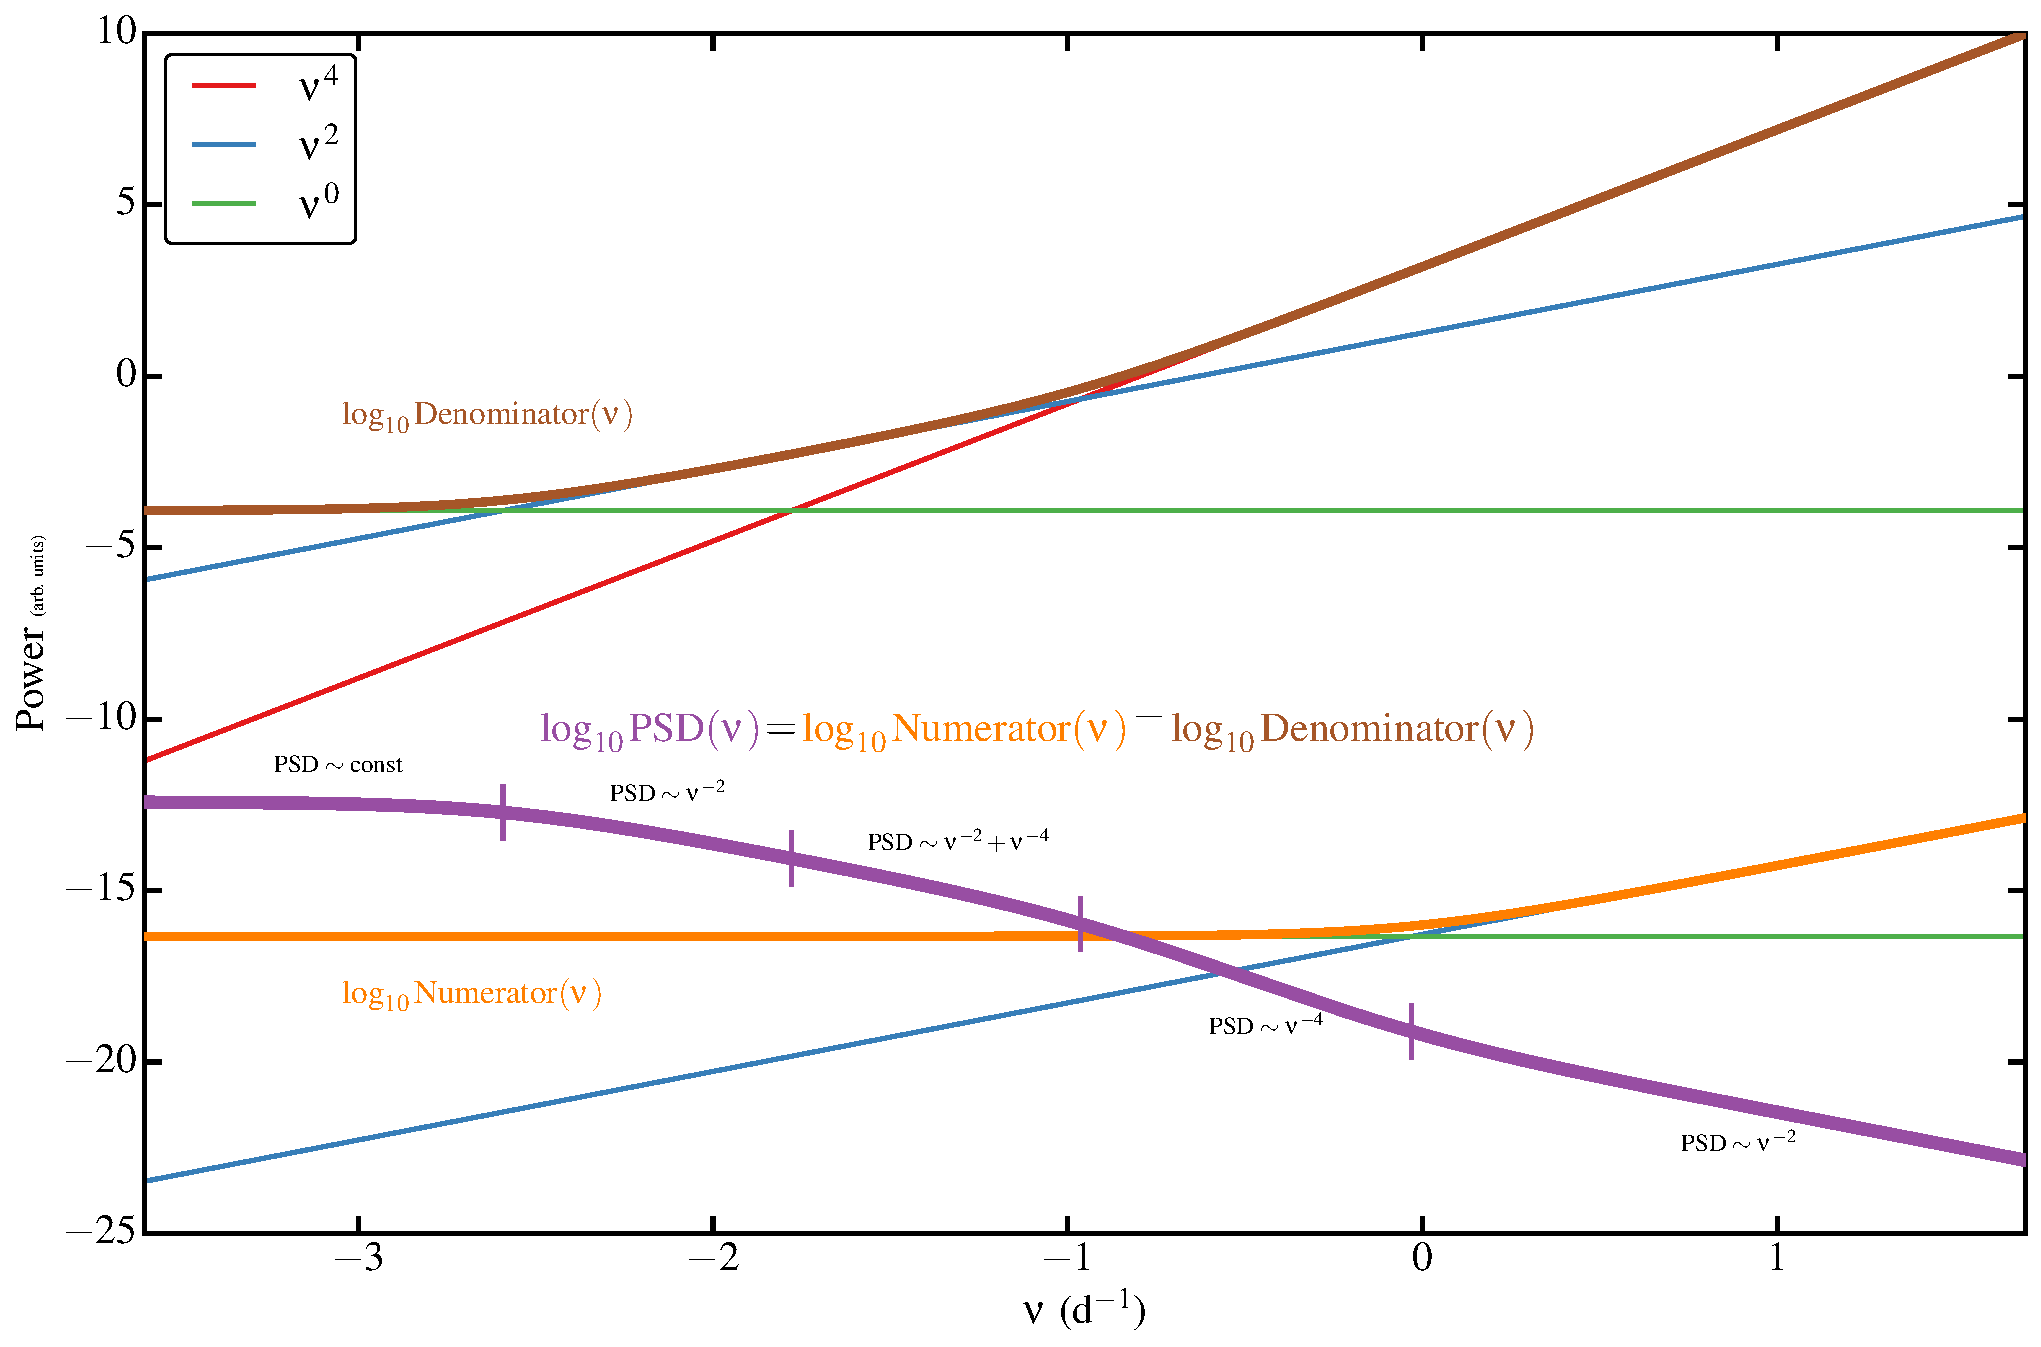
\includegraphics[width=5.0in]{figs/agn/AGN_Variability_01.pdf}
\caption{Behavior of the spectral index of the PSD (black) of the Kepler Sy1 
AGN Zw 229-15. This AGN is well-modelled by a C-ARMA(2,1) process. The spectral index varies
from 0 to 4 depending upon the frequency. Insufficient sampling of the light
curve (e.g. a few times a month), can result in the erroneous conclusion that a 
damped random walk (DRW) model (max spectral slope 2), adequately 
characterizes the variability.
}
\label{PSDvsFreq}
\end{figure}

Determination of the hyperparmeters that describe the PSD requires high frequency
sampling of the light curve ($\sim 1$~d$^{-1}$). Figure \ref{PSDvsFreq} shows
the frequency dependence of the spectral index of the PSD (black) of the Kepler Sy 1 AGN 
Zw 229-15. The light curve of this AGN is well-modelled by a C-ARMA(2,1) 
model. The C-ARMA(2,1) is a higher order random walk than the 
Damped Random Walk (DRW) of \citet{Kelly09} which is a C-ARMA(1,0)
 model. Recent varaibility studies indicate that the simple C-ARMA(1,0) 
model is insufficient to model AGN variability because the spectral
 index of the C-ARMA(1,0)
model is mathematically constrained to be 2 \citep{Kelly14,Kasliwal15,Simm15}. 
The PSD (black line) is the ratio of an even polynomial numerator (orange line) to 
an even polynomial denominator (brown line). Different powers of frequency dominate
the PSD at different frequencies depending on the hyperparameters of the C-ARMA(2,1) model. It is
clear that in the case of this AGN, the light curve must be sampled on timescales {\em shorter} than 
$1$-$5$ days in order to observe the $\nu^{-4}$ behavior characteristic of a higher order random walk.

\begin{figure}
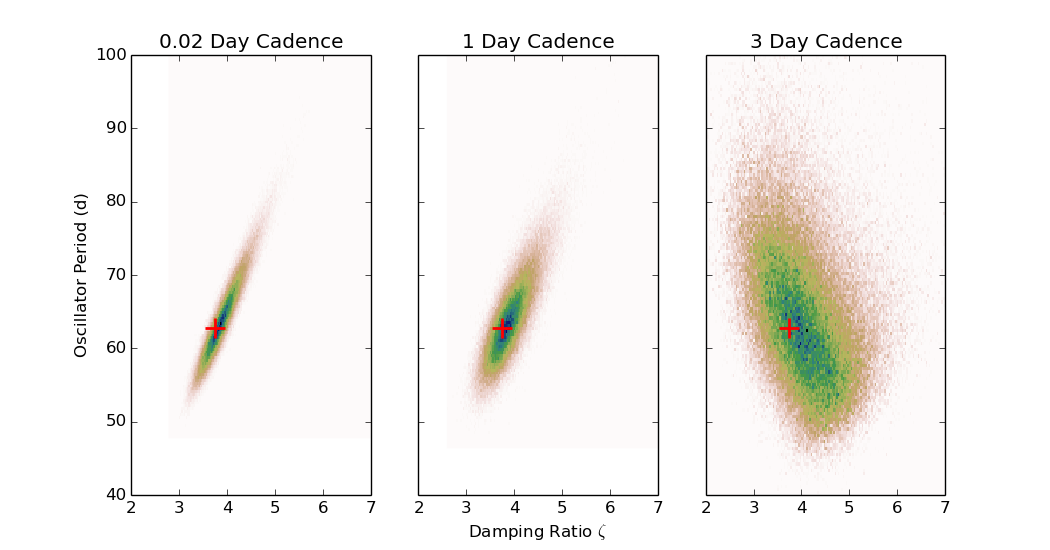
\includegraphics[width=5.0in]{figs/agn/AGN_Variability_00.png}
\caption{The effect of sampling cadence on hyperparameter estimation.}
\label{CadenceEffec}
\end{figure}

Accurate recovery of the PSD hyperparameters is greatly enhanced by rapid sampling. Figure \ref{CadenceEffect}
shows the effect of the sampling frequency on the inferred joint distribution of two
 hyperparameters of the C-ARMA(2,1) model, the 
oscillator timescale and the damping ratio. Degrading the sampling frequency from $1/$($30$~min) 
(Kepler) to $1/$($3$~d) changes both the size and the shape of the joint distribution i.e. it degrades both 
the accuracy and correlation of the inferred hyperparameters. 

The PRM measurements will probe the size and structure of the
accretion disk and BELR, in a statistical sense, and may provide
improved SMBH mass estimates for sources that have at least
single-epoch spectra. \new{Our goal is to understand the population of
AGN broad line regions, including their geometry. We expect to do this
via  a model that connects the BH mass, BLR geometry and AGN
photometric variability properties via a set of scaling relations. A
simple version of this is could be something like...\newline\newline
So, our target measurements are of $a$ and $b$, the X parameters.
Before we derive a metric that quantifies our ability to measure these
parameters, we can anticipate some of the sensitivity of the
photometric RM method to observing strategy.}

The PRM method is very sensitive to the sampling in each band,
therefore the ability to derive reliable time delays can be affected
significantly by the LSST cadence. The best results will be obtained
by having the most uniform sampling equally for each band.
Additionally, there is a trade-off between the number of DDFs and the
number of time delays that PRM can obtain \citep{CheloucheEtal2014}.
For example, an increase in the number of DDFs, with similarly dense
sampling in each field, can yield a proportionately larger number of
high-quality time delays, down to lower luminosities, but at the
expense of far fewer time delays (for relatively high luminosity
sources) in the main survey.

%\new{We focus on the PSD function as a way of characterizing AGN
%variability in various ways. What do we expect the AGN population to
%look like in PSD parameter space? The hyper-parameters that govern the
%relationships between PSD parameters and  AGN and host galaxy
%properties are probably of greatest scintific interest.}

% --------------------------------------------------------------------

\subsection{Metrics}
\label{sec:\secname:metrics}

Quantifying the response via MAF metrics: definition of the metrics,
and any derived overall figure of merit.

\new{In lieu of a simulated AGN population, we focus on a few
particular {\it diagnostic} metrics that capture  our likely ability
to measure the PSD across the population. These include: the
uniformity of the sampling pattern in log time lag?}


Need to compute the average and the dispersion in the
number of visits, per band, across the sky for the nominal OpSim
(during the entire survey). Since PRM works best for uniform sampling,
need to compare the distributions of the number of visits in each
band, averaged across the sky, and identify ways to minimize any
potential differences between these distributions. By running PRM
simulations, identify the 1) minimum number of visits (in any band)
that can yield any meaningful BELR-continuum lag estimates, and 2) the
largest difference in the number of visits between two different bands
that can yield any meaningful BELR-continuum lag estimates. Repeat
these simulations by doubling the nominal number of DDFs. Assess the
number of meaningful BELR-continuum time delays that can be obtained
with the nominal OpSim, and point out potential perturbations in the
cadence to improve the number and quality of such time delays.

% QPOs - Will the cadence and duration give you the proper range on the
% power spectrum to detect QPOs with a given mass, spin, and L/Ledd?
% (Bob Wagoner)


% --------------------------------------------------------------------

\subsection{OpSim Analysis}
\label{sec:\secname:analysis}

OpSim analysis: how good would the default observing strategy be, at
the time of writing for this science project?


% --------------------------------------------------------------------

\subsection{Discussion}
\label{sec:\secname:discussion}

Discussion: what risks have been identified? What suggestions could be
made to improve this science project's figure of merit, and mitigate
the identified risks?


% ====================================================================

\navigationbar


% --------------------------------------------------------------------

%% ====================================================================
%+
% SECTION:
%    section-name.tex  % eg lenstimedelays.tex
%
% CHAPTER:
%    chapter.tex  % eg cosmology.tex
%
% ELEVATOR PITCH:
%    Explain in a few sentences what the relevant discovery or
%    measurement is going to be discussed, and what will be important
%    about it. This is for the browsing reader to get a quick feel
%    for what this section is about.
%
% COMMENTS:
%
%
% BUGS:
%
%
% AUTHORS:
%    Phil Marshall (@drphilmarshall)  - put your name and GitHub username here!
%-
% ====================================================================

\section{Photometric Reverberation Mapping}
\def\secname{\chpname:photoRM}\label{sec:\secname}

\credit{ohadshemmer}

% This individual section will need to describe the particular
% discoveries and measurements that are being targeted in this section's
% science case. It will be helpful to think of a ``science case" as a
% ``science project" that the authors {\it actually plan to do}. Then,
% the sections can follow the tried and tested format of an observing
% proposal: a brief description of the investigation, with references,
% followed by a technical feasibility piece. This latter part will need
% to be quantified using the MAF framework, via a set of metrics that
% need to be computed for any given observing strategy to quantify its
% impact on the described science case. Ideally, these metrics would be
% combined in a well-motivated figure of merit. The section can conclude
% with a discussion of any risks that have been identified, and how
% these could be mitigated.

% A short preamble goes here. What's the context for this science
% project? Where does it fit in the big picture?

Photometric reverberation mapping (PRM), measuring the time-delayed
response of either the flux of the broad emission line region (BELR)
lines to the flux of the AGN continuum or between the continuum flux
in one (longer wavelength) band to the continuum flux in another (band
with shorter wavelength), will be one of the cornerstones of AGN
research in the LSST era (e.g., \citet{Chelouche2013};
\citet{CheloucheandZucker2013}; \citet{CheloucheEtal2014};
\citet{EdelsonEtal2015}; \citet{FausnaughEtal2015}). For example, LSST
is expected to deliver BELR line-continuum time delays in
$\sim10^5-10^6$ sources, which is unprecedented when compared to
$\sim50-100$ such measurements conducted via the traditional, yet much
more expensive (per source) spectroscopic method. Sources in the
deep-drilling fields (DDFs) will benefit from the highest quality PRM
time-delay measurements given the factor of $\sim10$ denser sampling.

% --------------------------------------------------------------------

\subsection{Target measurements and discoveries}
\label{sec:\secname:targets}

% Describe the discoveries and measurements you want to make.

% Now, describe their response to the observing strategy. Qualitatively,
% how will the science project be affected by the observing schedule and
% conditions? In broad terms, how would we expect the observing strategy
% to be optimized for this science?

The PRM measurements will probe the size and structure of the
accretion disk and BELR, in a statistical sense, and may provide
improved SMBH mass estimates for sources that have at least
single-epoch spectra. \new{Our goal is to understand the population of
AGN broad line regions, including their geometry. We expect to do this
via  a model that connects the BH mass, BLR geometry and AGN
photometric variability properties via a set of scaling relations. A
simple version of this is could be something like...\newline\newline
So, our target measurements are of $a$ and $b$, the X parameters.
Before we derive a metric that quantifies our ability to measure these
parameters, we can anticipate some of the sensitivity of the
photometric RM method to observing strategy.}

The PRM method is very sensitive to the sampling in each band,
therefore the ability to derive reliable time delays can be affected
significantly by the LSST cadence. The best results will be obtained
by having the most uniform sampling equally for each band.
Additionally, there is a trade-off between the number of DDFs and the
number of time delays that PRM can obtain \citep{CheloucheEtal2014}.
For example, an increase in the number of DDFs, with similarly dense
sampling in each field, can yield a proportionately larger number of
high-quality time delays, down to lower luminosities, but at the
expense of far fewer time delays (for relatively high luminosity
sources) in the main survey.

% --------------------------------------------------------------------

\subsection{Metrics}
\label{sec:\secname:metrics}

Quantifying the response via MAF metrics: definition of the metrics,
and any derived overall figure of merit.


Need to compute the average and the dispersion in the
number of visits, per band, across the sky for the nominal OpSim
(during the entire survey). Since PRM works best for uniform sampling,
need to compare the distributions of the number of visits in each
band, averaged across the sky, and identify ways to minimize any
potential differences between these distributions. By running PRM
simulations, identify the 1) minimum number of visits (in any band)
that can yield any meaningful BELR-continuum lag estimates, and 2) the
largest difference in the number of visits between two different bands
that can yield any meaningful BELR-continuum lag estimates. Repeat
these simulations by doubling the nominal number of DDFs. Assess the
number of meaningful BELR-continuum time delays that can be obtained
with the nominal OpSim, and point out potential perturbations in the
cadence to improve the number and quality of such time delays.

% --------------------------------------------------------------------

\subsection{OpSim Analysis}
\label{sec:\secname:analysis}

OpSim analysis: how good would the default observing strategy be, at
the time of writing for this science project?


% --------------------------------------------------------------------

\subsection{Discussion}
\label{sec:\secname:discussion}

Discussion: what risks have been identified? What suggestions could be
made to improve this science project's figure of merit, and mitigate
the identified risks?


% ====================================================================

\navigationbar


% --------------------------------------------------------------------

% ====================================================================
%+
% SECTION:
%    AGN_Microlensing.tex
%
% CHAPTER:
%    AGN.tex
%
% ELEVATOR PITCH:
%    Using AGN microlensing to measure the size and structure of
%    accretion disks. Depends on well-sampled multi-filter light curves,
%    and a large sample of detected strongly-lensed AGN.
%
% COMMENTS:
%
%
% BUGS:
%
%
% AUTHORS:
%    Timo Anguita (@tanguita)
%-
% ====================================================================

\section{AGN Size and Structure with Microlensing}
\def\secname{\chpname:microlensing}\label{sec:\secname}

\credit{tanguita}

% This individual section will need to describe the particular
% discoveries and measurements that are being targeted in this section's
% science case. It will be helpful to think of a ``science case" as a
% ``science project" that the authors {\it actually plan to do}. Then,
% the sections can follow the tried and tested format of an observing
% proposal: a brief description of the investigation, with references,
% followed by a technical feasibility piece. This latter part will need
% to be quantified using the MAF framework, via a set of metrics that
% need to be computed for any given observing strategy to quantify its
% impact on the described science case. Ideally, these metrics would be
% combined in a well-motivated figure of merit. The section can conclude
% with a discussion of any risks that have been identified, and how
% these could be mitigated.

% A short preamble goes here. What's the context for this science
% project? Where does it fit in the big picture?

Microlensing due to stars projected on top of individual
gravitationally-lensed quasar images produce additional magnification.
Using the fact that the Einstein radii of stars in lensing galaxies
closely match the scales of different emission regions in
high-redshift AGNs (micro-arcseconds), analyzing microlensing induced
flux variations statistically on individual systems allows us to
measure ``sizes'' of AGN regions.

Assuming a thermal profile for accretion disks, sizes in different
emission wavelengths will be probed and as such, constraints on the
slope of this thermal profile will be placed. Given the sheer number
of lensed systems that LSST is expected to discover ($\sim8000$),
this will allow us to stack systems for better constraints and
hopefully determine the {\it evolution of the size and profile.} Due to the
typical relative velocities of lenses, microlenses, observers (Earth)
and source AGN, the microlensing variation timescales are between
months to a few decades.


% --------------------------------------------------------------------

\subsection{Target measurements and discoveries}
\label{sec:\secname:targets}

% Describe the discoveries and measurements you want to make.

% Now, describe their response to the observing strategy. Qualitatively,
% how will the science project be affected by the observing schedule and
% conditions? In broad terms, how would we expect the observing strategy
% to be optimized for this science?

\new{Our goal is to understand the population of AGN accretion disk sizes
and profiles. We anticipate doing this via a hierarchical model where
these properties are related to each other in some way, perhaps via
power law scaling relations. A very simple version of this is the following...
\newline\newline
So, our targets are the parameters $a$ and $b$, that describe this
simple population. How well will we be able to measure these, for a
given survey strategy? This is what our MAF metric will quantify.
Before we design this, we can predict the likely sensitivities of this
measurement.}


The quasar microlensing optical depth is $\sim1$, so every lensed
quasar should be affected by microlensing at any given point in time.
However, measurable variability can occur on longer timescales.
\citet{MosqueraandKochanek2011} studied all known lensed quasars.
They found the median timescale between high magnification events
(Einstein crossing time scales) in the observed $I$-band is of the
order of $\sim20$~yr (with a distribution between 10 and 40~yr).
However, the source crossing time (duration of a high magnification
event) is $\sim7.3$~months (with a distribution tail up to 3~yr).
This basically means that out of all the lensed quasar {\em images}
(microlensing between images is completely uncorrelated) about half
of them will be quiescent during the 10~yr baseline of LSST. However,
since the typical number of lensed images is either two or four, it
means that, statistically, in every system, one (for doubles) or two
(for quads) high magnification events should be observed in 10~yr of
LSST monitoring.

Note that, the important cadence parameter is the source crossing time,
as it is the length of the event to be as uniformly sampled as
possible. The 7.3 months crossing time is the median for the observed
$i$-band, but this time would be significantly shorter for bluer bands:
for a thermal profile with slope
$\alpha: R_\lambda \propto \lambda^\alpha$ implies source crossing time
$t_{\rm s} \propto \lambda^{1/\alpha} \rightarrow
t_u=t_i \times (\lambda_{\rm u} / \lambda_{\rm i})^{1/\alpha}$. For a
Shakura-Sunyaev slope of $\alpha=0.75$ this would correspond to
$7.3 \times (3600/8140)^{4/3}$ months which is $\approx 2.5$ months in
the $u$-band.

In terms of the cadence, at least three evenly sampled data points per
band within two to three months would be preferred to be able to map
the constraining high magnification event(?), and these would
hopefully be uniformly spaced. Very tight cadence (e.g., DDFs) would
increase the constraints significantly. However, since lensed quasars
are not that common, this smaller area would mean only a few
($\sim80$?) suitable systems monitored in the DDFs.

Regarding the season length, the ``months'' timescale of high
magnification events very likely means that we can/will miss high
magnification events in the season gaps, at least in the bluer bands.

Show stopper: observations spread on timescales larger than 3 months(?).
This would likely miss the high magnification events. In those cases
we could perhaps consider close consecutive photometric bands as
equivalent accretion disk regions, however this would mean weaker
constraints on the thermal profile.
%
Important Note: all this science needs to be done on lensed quasars
with measured or very short time delays to remove the intrinsic
variability signal, which might significantly reduce the sample.

{\bf Microlensing Aided Reverberation Mapping:} Given that
microlensing mostly affects continuum emission rather than BELR line
emission, microlensing may enable disentangling the BELR line plus the
continuum emission in single photometric bands, allowing the use of
single broad band PRM measurements \citep{SluseandTewes2014}. As with
the two-band PRM method discussed above, the denser (and the longer)
the sampling, the more accurate are the constraints that can be
obtained for the time delays.

% --------------------------------------------------------------------

\subsection{Metrics}
\label{sec:\secname:metrics}

Quantifying the response via MAF metrics: definition of the metrics,
and any derived overall figure of merit.

Need to compute the dispersion in the time gap
between visits in the same band, across the sky, in order to assess
the fraction of microlensing events that might be missed (on top of
seasonal gaps).

% microlensing - convolve microlensing timescales for QSOs we already know
% about. how many of the high magnification events do we get? How bright?
% @tanguita

% --------------------------------------------------------------------

\subsection{OpSim Analysis}
\label{sec:\secname:analysis}

OpSim analysis: how good would the default observing strategy be, at
the time of writing for this science project?


% --------------------------------------------------------------------

\subsection{Discussion}
\label{sec:\secname:discussion}

Discussion: what risks have been identified? What suggestions could be
made to improve this science project's figure of merit, and mitigate
the identified risks?


% ====================================================================

\navigationbar


% --------------------------------------------------------------------

\subsection{Discussion}
\label{sec:\secname:discussion}

% Discussion: what risks have been identified? What suggestions could be
% made to improve the figures of merit, and mitigate the identified risks?
% What ``tweaks'', if any, can be proposed to the nominal LSST observing strategy
% in order to help achieve key AGN science goals?

Some additional considerations/thoughts that came up during the workshop:

1) Assuming we will have 10 DDFs, perhaps one of those fields could be
sampled more heavily than the others and would be visited nightly (or
even more frequently, e.g., from $\sim1$ to $\sim1000$ min) per band.
This can be justified by the fact that
a) very few AGNs have been monitored at these frequencies on such a
long baseline, leaving room for discovery, and b) this may probe
intermediate-mass black holes ($\sim10^4 - 10^5$~$M_{\odot}$) via PRM or
PSDs. Good candidate fields are the CDF-S and the MCs.
Need to suggest a strategy for an OpSim (or commissioning).

2) Need to assess the effects of the LSST cadence on the ability to
detect periodic AGNs and quasi-periodic oscillations (QPOs) in AGNs.

3) Needs from OpSim: in order to have informative metrics, we need to have
accurate model light curves that can reproduce how the fiducial light
curves appear in different bands, at different inherent luminosities,
and at different redshifts.

% DDF - we need longer duration OpSims in these fields. (Bob Wagoner)
% (https://github.com/LSSTScienceCollaborations/ObservingStrategy/blob/master/opsim/README.md)

% commissioning opportunity - one field, one night, one filter (u or g).
% 15/30 sec exposures. (Bob Wagoner)
% (https://github.com/LSSTScienceCollaborations/ObservingStrategy/blob/master/commissioning/README.md)

\todo{}{Compare the current science content with the AGN chapter in the
Science Book as well as with the Ivezic et al. overview paper
(http://arxiv.org/pdf/0805.2366v4.pdf).}

\todo{}{Compare the $Y$-band (and other bands) depths, single
epoch and final co-added, from  enigma\_1189 with other OpSims.}

\todo{}{Assess the effect of non-simultaneous colors on AGN selection.}

\todo{}{Based on the current OpSim, need to specify the magnitude limits
at the highest airmass and assess the limitations of the DCR method in
the $L-z$ plane. Should check this with MAF and if indeed AM <= 1.4, need
to add a request in:
https://github.com/LSSTScienceCollaborations/ObservingStrategy/tree/master/opsim
}

\todo{}{Assess whether, e.g., a pair of $\sim2.5$ min exposures (i.e., $\sim10$
times longer than the standard exposures) at airmass $\sim2$ would get deep
enough for useful DCR constraints for a large fraction of the AGNs. This may
be a non-negligible perturbation of the expected 56-184 visits per band, and
may even be impossible given current upper limits on exposure times, but
this would help improve photo-z's for galaxies and SNe too.}

\todo{}{For PRM and microlensing: obtain distributions (mean and dispersion)
of the number of visits, per band, across the sky for the nominal OpSim
(during the entire survey).}

\todo{}{Add a discussion about blazars and LSST cadence (e.g., Isler+15?).
Would blazar science benefit from a specific cadence requirement?}

\todo{}{Check the Astrometry chapter and assess the astrometric precision
for AGN selection. For example, we may require very good depth at least in
the 1st and 10th year of the survey.}

\todo{}{Indicate the properties (frequency range and sampling) for obtaining
optimal PSDs required for QPO detection (given MBH, spin, and L/LEdd). Based on
current OpSim, assess the potential of discovering QPOs in the main survey
and in the DDFs.}

\navigationbar
